\pagenumbering{arabic}
%\documentclass[slides]{beamer}
\documentclass[mathserif]{beamer}
\usepackage[framesassubsections]{beamerprosper}
\setbeamercovered{transparent}
%\documentclass[slides,hyperref={pdfpagelabels=false}]{beamer}
%\documentclass[handout,gray]{beamer}
\usepackage[T1]{fontenc}
\usepackage[utf8]{inputenc}
\usepackage{textcomp}
\usepackage{verbatim}
\usepackage{amsbsy}
\usepackage{multirow}
\usepackage{multicol}
\usepackage{booktabs} % Make some nice tables
\usepackage{ae,aecompl}

%%%%%%%%%%%% COULEURS %%%%%%%%%%%%%%%%%%%%%%%%%%%

\mode<presentation>
{
  \definecolor{beamerstructure}{RGB}{43,79,112}
  \definecolor{sidebackground}{RGB}{230,242,250}
  \definecolor{CTCC}{RGB}{133,188,228}
  \color{beamerstructure}
  \usetheme{default}
  \usepackage{courier}
  \beamertemplateballitem
\setbeamertemplate{navigation symbols}{}
%\setbeamertemplate{sidebar left}{\thispdfpagelabel{\insertframenumber}}
%\setbeamertemplate{footline}{\quad\insertframenumber}
%\usecolortheme{CTCC}
}
\usebackgroundtemplate{\includegraphics[width=1.02\paperwidth]{../templets/ctcc_general.jpg}}

\title{\\\vspace{1cm}
Real-space all-electron Density Functional Theory \\
with Multiwavelets}
%\subtitle{\textcolor{magenta}{My subtitle (if applicable)}}
\author{Stig Rune Jensen}
\institute[CTCC]{\\[-6mm]stig.r.jensen@uit.no\\[6mm]UiT The Arctic University of Norway\\[6mm]
\includegraphics[height=1.5cm]{../templets/uio.pdf}\hspace{1cm} 
\includegraphics[height=1.5cm]{../templets/sff.pdf}\hspace{1cm}
\includegraphics[height=1.5cm]{../templets/uit.pdf}}
\date{Troms\o, March 20th 2014}

\newcommand{\gb}[1]{green!#1!black}
\newcommand{\rb}[1]{red!#1!black}
\newcommand{\bb}[1]{blue!#1!black}
\newcommand{\coleq}{red!60!black}
\newcommand{\du}{\textrm{d}}

\newcommand{\mydef}{\stackrel{\text{def}}{\hbox{=}}} 

\begin{document}

\footnotesize
\setlength{\unitlength}{\textwidth}

{
\usebackgroundtemplate{\includegraphics[width=1.02\paperwidth]{../templets/ctcc_forside.jpg}}
\maketitle
}

\begin{frame}
    \frametitle{Outlook}
    \begin{itemize}
	\item	Multiwavelets
	\begin{itemize}
	    \item   Functions
	    \item   Operators
	    \item   Paper I
	\end{itemize}
	\item	Parallelization
	\begin{itemize}
	    \item   Shared memory
	    \item   Distributed memory
	    \item   Paper II
	\end{itemize}
	\item	Density Functional Theory
	\begin{itemize}
	    \item   Integral formulation
	    \item   Iterative algorithm
	    \item   Paper III
	\end{itemize}
    \end{itemize}
\end{frame}

\begin{frame}
    \frametitle{Multiwavelets}
    Scaling/wavelet functions
\end{frame}

\begin{frame}
    \frametitle{Multiwavelets}
    Function representation\\
    Projection of orbital
\end{frame}

\begin{frame}
    \frametitle{Multiwavelets}
    Paper I
\end{frame}

\begin{frame}
    \frametitle{Parallel programming}
    Why parallel processing?
    \begin{itemize}
	\item	To get more processing power
	\item	To get more available memory
	\item	Future $\rightarrow$ \emph{more} processors rather than faster
    \end{itemize}
    \ \\
    \ \\
    \ \\
    Parallelization means
    \begin{itemize}
	\item	\textbf{distributing work} to processors
	\item	\textbf{syncronization} of distributed work
	\item	\textbf{distributing data} (if memory is distributed)
	\item	\textbf{communication} of distributed data
    \end{itemize}
\end{frame}

\begin{frame}
    \frametitle{Shared memory parallelization (OpenMP)}
    \begin{minipage}[b]{0.45\linewidth}
	Pros
	\begin{itemize}
	    \item Relatively simple implementation
	    \item Quick way to good performance
	    \item No communication
	    \item Simple load balance
	\end{itemize}
	Cons
        \begin{itemize}
	    \item Small to medium scale parallelization
	    \item Limited memory
	    \item Race conditions
	    \item Tedious debugging (Heisenbugs)
	\end{itemize}
    \end{minipage}
    \hfill
    \begin{minipage}[b]{0.4\linewidth}
	\includegraphics[bb = 120 160 460 450, clip, scale=0.4]{figures/parallel_OMP.pdf}
	\ \\
	\ \\
	\ \\
	\ \\
    \end{minipage}
\end{frame}

\begin{frame}
    \frametitle{Distributed memory parallelization (MPI)}
    \begin{minipage}[b]{0.45\linewidth}
	Pros
	\begin{itemize}
	    \item Large scale parallelization
	    \item Extensive memory
	\end{itemize}
	Cons
	\begin{itemize}
	    \item Complicated implementation
	    \item User specified work/data decomposition 
	    \item User specified communication
	    \item Difficult to load balance
	    \item Communication overhead
	\end{itemize}
    \end{minipage}
    \hfill
    \begin{minipage}[b]{0.4\linewidth}
	\only<1>{\includegraphics[bb = 120 160 460 450, clip, scale=0.4]{figures/parallel_MPI_1.pdf}
	\ \\
	}
	\only<2>{\includegraphics[bb = 120 160 460 450, clip, scale=0.4]{figures/parallel_MPI_2.pdf}
	\ \\
	}
    \end{minipage}
\end{frame}

\begin{frame}
    \frametitle{Parallel efficiency}
    The overall parallel efficiency is given by
    \begin{itemize}
	\item Ideal efficiency (Amdahl's law)
	\item Synchronization (load imbalance) 
	\item Communication overhead (must be parallelized as well)
    \end{itemize}
    \only<1>{\includegraphics[bb = 00 250 500 630, scale=0.9]{figures/amdahl.pdf}}
    \only<2>{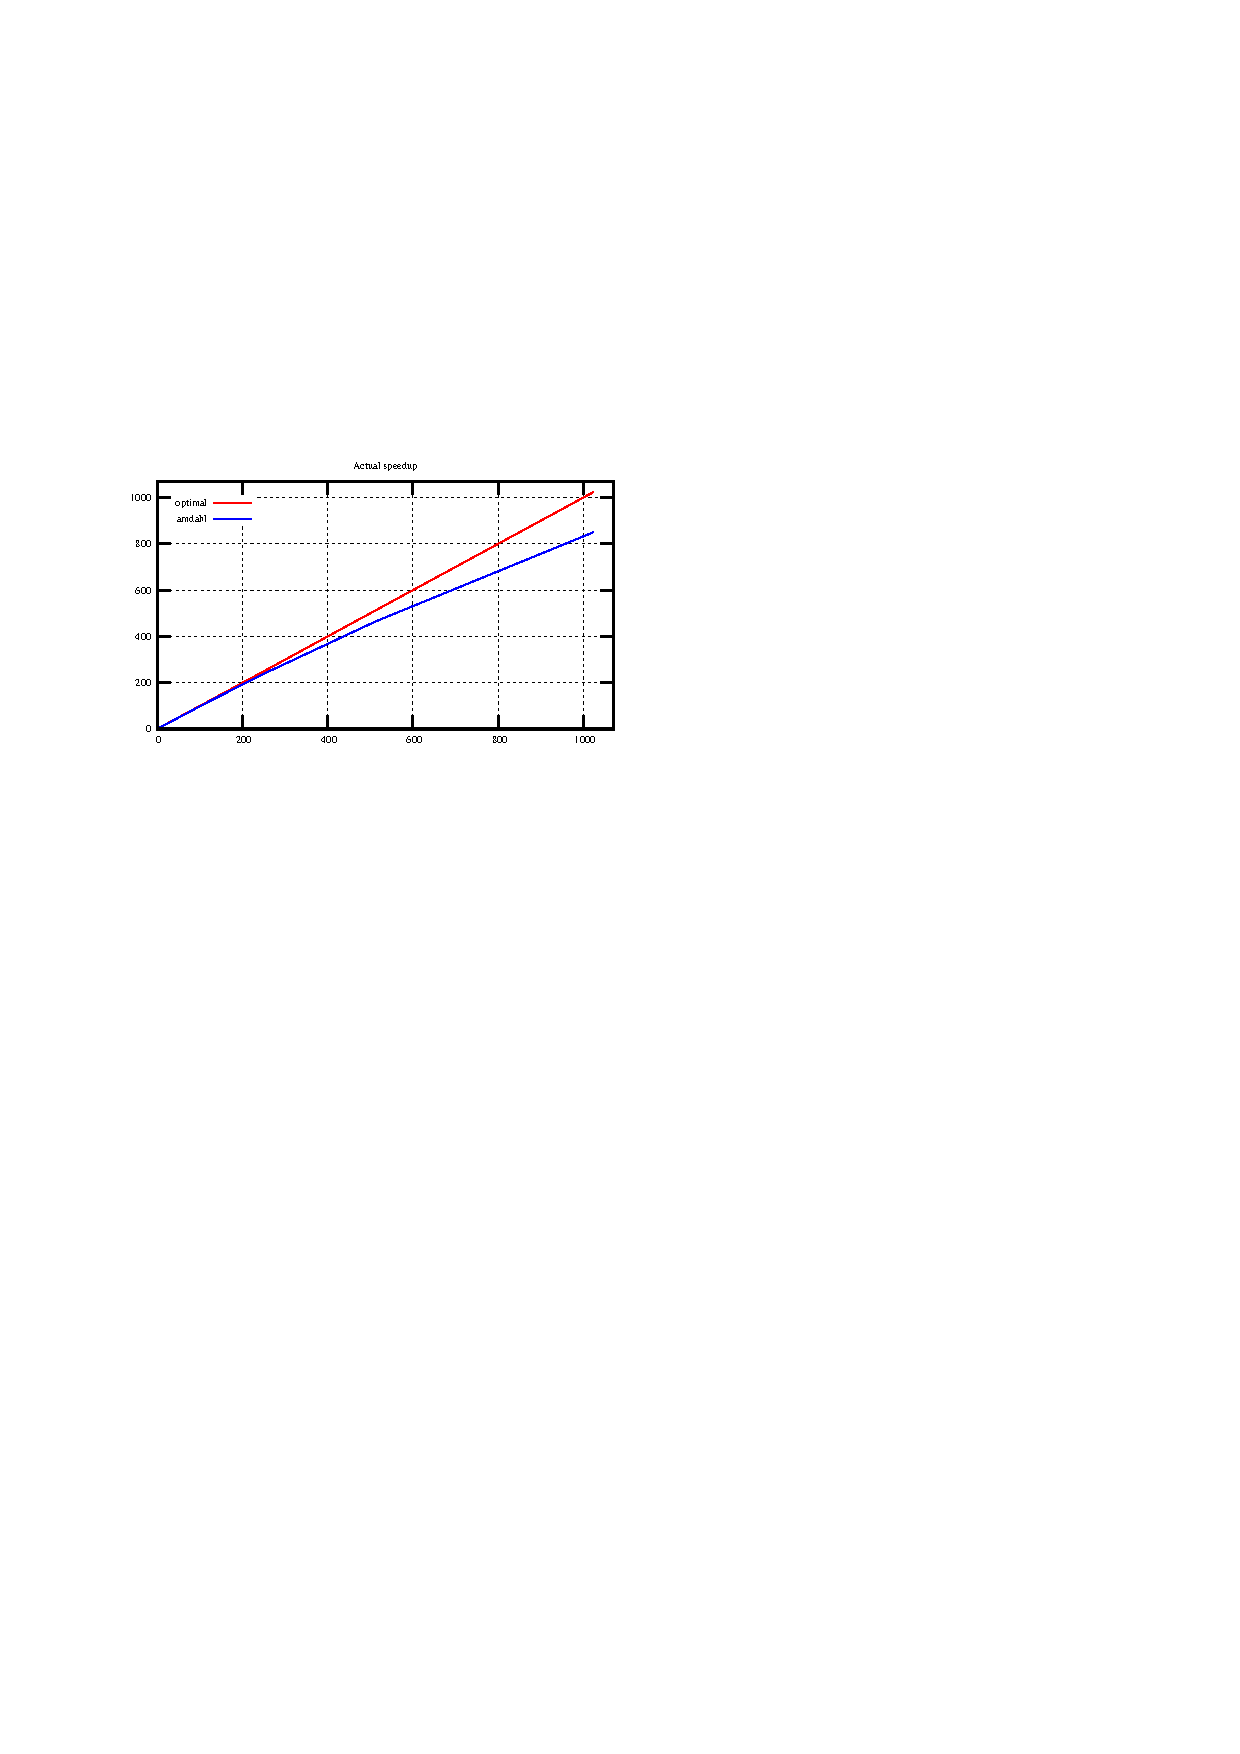
\includegraphics[bb = 00 250 500 630, scale=0.9]{figures/mpiAmdahl_1.pdf}}
    \only<3>{\includegraphics[bb = 00 250 500 630, scale=0.9]{figures/mpiAmdahl_2.pdf}}
    \only<4>{\includegraphics[bb = 00 250 500 630, scale=0.9]{figures/mpiAmdahl_3.pdf}}
    \only<5>{\includegraphics[bb = 00 250 500 630, scale=0.9]{figures/mpiAmdahl_4.pdf}}
\end{frame}

\begin{frame}
    \frametitle{Data distribution}
    Domain decomposition using Hilbert path
    \only<1>{\includegraphics[bb = 70 700 400 800, scale=1.0, clip]{figures/hilbertCurve.pdf}}
    \only<2>{\includegraphics[bb = 70 590 400 690, scale=1.0, clip]{figures/hilbertCurve.pdf}}
\end{frame}

\begin{frame}
    \frametitle{Multiwavelets}
    Operator representation\\
    Separation of variables\\
    Vanishing moments\\
    Plot of separated 1/r
\end{frame}

\begin{frame}
    \frametitle{Multiwavelets}
    Paper II
\end{frame}

\begin{frame}
    \frametitle{Linear scaling Coulomb interaction}
    Linear scaling results
\end{frame}

\begin{frame}
    \frametitle{Linear scaling Coulomb interaction}
    Parallel results
\end{frame}

\begin{frame}
    \frametitle{Density Functional Theory}
\end{frame}

\begin{frame}
    \frametitle{Computational chemistry}
    Basis sets
\end{frame}

\begin{frame}
    \frametitle{Integral formulation}
    Canonical equations
\end{frame}

\begin{frame}
    \frametitle{Algorithm}
    Mention fixed lambda\\
    Mention KAIN
\end{frame}

\begin{frame}
    \frametitle{One-electron systems}
    Convergence plot\\
    Orbital plots
\end{frame}

\begin{frame}
    \frametitle{Many-electron systems}
    Convergence plots\\
    Accuracy plots
\end{frame}

\begin{frame}
    \frametitle{Orbital localization}
    Non-canonical equations\\
    Orbital plots\\
    Convergence table
\end{frame}

\begin{frame}
    \frametitle{Summary}
\end{frame}

\begin{frame}
    \frametitle{Acknowledgments}
    Chemistry:
    \begin{itemize}
	\item Luca Frediani
    \end{itemize}
    \ \\
    \ \\
    High performance computing:
    \begin{itemize}
    	\item Jonas Juselius
    	\item Peter Wind
	\item NOTUR
    \end{itemize}
    \ \\
    \ \\
    Mathematics:
    \begin{itemize}
	\item Tor Fl\aa
	\item Antoine Durdek
    \end{itemize}
    \ \\
    \ \\
    \ \\
    Contact:
    \begin{itemize}
	\item stig.r.jensen@uit.no
    \end{itemize}
\end{frame}

\end{document}
